\ylDisplay{Prillid} % Ülesande nimi
{Autor} % Autor
{lõppvoor} % Voor
{2011} % Aasta
{P 8} % Ülesande nr.
{3} % Raskustase
{
% Teema: Valgusõpetus
\ifStatement
Juku on lühinägelik ja kasutab prille optilise tugevusega $D_1 = -4$ dpt. Ükskord proovis ta oma prillide asemel ette vanaema lugemisprille, mille optiline tugevus on $D_2 = +4$ dpt. Juku märkas, et vanaema prille kandes läheb pilt veel udusemaks, kuid neid peast teatud kaugusel hoides näeb ta ka kaugeid objekte teravalt. Mis oli prillide suurim kaugus silmast, mille korral Juku veel kaugeid objekte teravalt nägi? Mis oli läbi vanaema prillide nähtud pildi juures ebaharilik? Prille tavapärasel viisil kandes on silma kaugus prilliklaasist tühiselt väike.
\fi
\ifHint
Lühinägelik silm näeb teravalt objekti, mis asub ei asu kaugmal teatud vahemaast. Prillide eesmärgiks on kaugest objektist tekitada kujutis, mis asub silmast samal kaugusel. Lõpmata kaugelt objektilt tulevad kiired on paralleelsed ja kujutise kaugus läätsest on võrdne fookuskauguse absoluutväärtusega.
\fi
\ifSolution
\begin{center}
	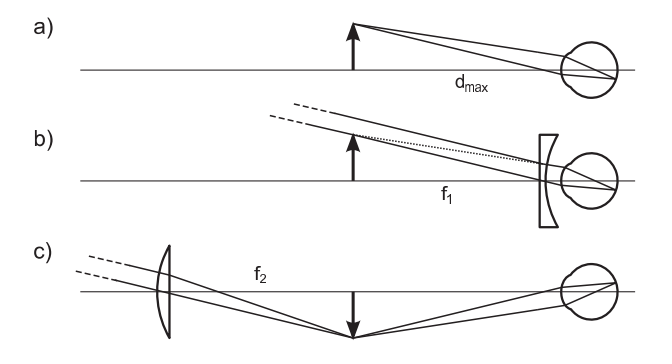
\includegraphics[width=0.5\linewidth]{2011-v3p-08-lah.PNG}
\end{center}
Lühinägelik silm näeb teravalt objekti, mis asub ei asu kaugmal teatud vahemaast $d_{max}$ (joon. a). Prillide eesmärgiks on kaugest objektist tekitada kujutis, mis asub silmast samal kaugusel (joon. b). Lõpmata kaugelt objektilt tulevad kiired on paralleelsed ja kujutise kaugus läätsest on võrdne fookuskauguse absoluutväärtusega $\mid f_1 \mid = \frac{1}{\mid D_1 \mid}$ . Silma kaugus prilliklaasist on väike ja $d_{max} \approx \mid f_1 \mid$. Kumerlääts lugemisprillides tekitab kauge objekti tõelise kujutise (joon. c), mille kaugus läätsest on $\mid f_2 \mid = \frac{1}{\mid D_2 \mid}$ . Silma kaugus lugemisprillidest on 
\begin{center}
$l = \mid f_2 \mid + d_{max} \approx \mid f_2| \mid + \mid f_1 \mid = \frac{1}{\mid D_2 \mid + \mid D_1 \mid}$ .
\end{center}
Pannes valemisse arvud sisse, saame $l = 0,5 m = 50$ cm. Sellisel ebaharilikul viisil prille kasutades on kujutis pööratud.
\fi
}
